\documentclass[a4paper,12pt]{article}

\usepackage[utf8x]{inputenc}
\usepackage[english,ngerman]{babel}
\selectlanguage{ngerman}

\usepackage[T1]{fontenc}
\usepackage{amsmath}
\usepackage{graphicx}
\usepackage{graphviz}

\usepackage{amsfonts}

\usepackage{url}
\usepackage[colorlinks=false,pdfborder={0 0 0},breaklinks=true]{hyperref}


\begin{document}

\title{DAT-Projekt Lichtsteuerung}
\author{Marius \textbf{Schuller}\\
        Stefan \textbf{Thiemann}\\
		Patrick \textbf{Wildt}}
\maketitle

\tableofcontents

\newpage

\noindent
Hier wird kurz die Grundidee des Schwerpunktprojekts, sowie welche Hardware 
benötigt wird, beschrieben.

\section{Einführung}
\label{einfuehrung}

Im Zuge der Internet-of-Things-Kampagne\footnote{\url{http://www.nextgenerationmedia.de}}
werden immer mehr ``dumme'' bzw. einfache Geräte miteinander vernetzt und die
resultierenden Daten intelligent miteinander verknüpft. Dazu gehören auch Lichter und
Glühbirnen. Zur Vernetzung und Steuerung der Lichter existieren bereits mehrere
aktuelle Technologien. Mit Hilfe einer der standardisierten Technologie möchten wir
einen Controller implementieren, welcher diese Lichter kontrollieren kann.

\section{Lichtsteuerungs-Technologien}
\label{technology}

Üblicherweise möchten Hersteller ein eigenes Produkt-Ökosystem erstellen, aus dem ein
Anwender nicht oder nur schwer entkommen kann. Hierfür werden von den Herstellern
eigene, unfreie Protokolle implementiert. Beispielsweise bietet \textit{LimitlessLED}
\footnote{\url{http://www.limitlessled.com}} Glühbirnen, welche sich
über 2,4 GHz WLAN in das lokale Netzwerk verbinden. Für die eigentliche
Steuerung wurde dazu eine eigene API entwickelt. Eine weitere bekannte Technologie
zur Steuerung von Geräten ist \textit{Bluetooth}. Hier ist es derzeit möglich
mit Hilfe des \textit{Generic Attribute Profile}, kurz
\textit{GATT}\footnote{\url{https://de.wikipedia.org/wiki/Bluetooth-Profile}},
ein eigenes Protokoll zu sprechen. Dies wird bei mehreren smarten Glühbirnen
verwendet um ein proprietäres Lichtsteuerungsprotokoll zu implementieren.

Die \textit{Bluetooth} Konkurrenten
\textit{Z-Wave}\footnote{\url{http://www.z-wavealliance.org}}, welches sich auf das
so genannte \textit{Home Control}-Szenario konzentriert, sowie
\textit{ZigBee}\footnote{\url{http://www.zigbee.org}},
implementieren wieder jeweils eigene Lichtprotokolle. Diese Protokolle sind jedoch
für jeden Client des Funkstandards nutzbar, sodass die Hersteller kein
eigenes Protokoll implementieren mussten. Der Funkstandard \textit{ZigBee} wird
von den namhaften Herstellern \textit{Philips} und \textit{Osram} verwendet.

Für das Schwerpunktprojekt würden wir uns auf \textit{ZigBee} kompatible Geräte
konzentrieren. Vor allem die Produkte der \textit{Philips hue} Reihe.

\section{Komponenten}
\label{components}

Die eigentliche Logik zur Steuerung der Lichter kann auf einem \textit{RaspberryPi}
implementiert werden. Um den Funkstandard \textit{ZigBee} sprechen zu können wird ein
kompatibles Funkmodul benötigt. Hierfür kann das \textit{RaspBee}-Modul verwendet werden.
Dieses gibt es in zwei Varianten, \textit{Basic} und \textit{Premium}. Während man mit der
Basic-Variante nur mit 5 Knoten sprechen darf, ist dies bei der Premium-Variante
unbegrenzt. Die Lichter würden aus einem \textit{Philips Hue} Starterkit bestehen.

\section{Hardware}
\label{hardware}

\subsection{RaspBee Premium, Raspberry-Pi Einzeln}

\begin{tabular}{p{2cm}p{4.5cm}p{3cm}p{3cm}}
   Menge & Produkt & Einzelpreis & Gesamtpreis\\
   \hline
   3 & \href{http://www.conrad.de/ce/de/product/1316978/Raspberry-Pi-2-Model-B-1-GB-ohne-Betriebssystem}{RaspberryPi 2} & 42 Euro & 126 Euro\\
   3 & \href{http://www.conrad.de/ce/de/product/1369407/Raspberry-Pi-Erweiterungs-Platine-Zigbee-200-Knotenpunkte-Raspberry-Pi}{RaspBee Premium} & 60 Euro & 180 Euro\\
   3 & \href{http://www.conrad.de/ce/de/product/1314141/Philips-Hue-LED-Leuchtmittel-Erweiterung-E27-9-W-RGB}{Philips Hue LED}
        \newline 1 x 9W A60 E27 & 59 Euro & 177 Euro\\
   \hline
   Gesamtpreis & & & \textbf{483 Euro}\\
\end{tabular}

\subsection{RaspBee Premium, Raspberry-Pi Bundle}

\begin{tabular}{p{2cm}p{4.5cm}p{3cm}p{3cm}}
   Menge & Produkt & Einzelpreis & Gesamtpreis\\
   \hline
   3 & \href{http://www.reichelt.de/Einplatinen-Computer/RASP-2-B-ALL-IN/3/index.html?ACTION=3&GROUPID=6666&ARTICLE=152855}{RaspberryPi 2 Bundle} & 70 Euro & 210 Euro\\
   3 & \href{http://www.conrad.de/ce/de/product/1369407/Raspberry-Pi-Erweiterungs-Platine-Zigbee-200-Knotenpunkte-Raspberry-Pi}{RaspBee Premium} & 60 Euro & 180 Euro\\
   3 & \href{http://www.conrad.de/ce/de/product/1314141/Philips-Hue-LED-Leuchtmittel-Erweiterung-E27-9-W-RGB}{Philips Hue LED}
        \newline 1 x 9W A60 E27 & 59 Euro & 177 Euro\\
   \hline
   Gesamtpreis & & & \textbf{567 Euro}\\
\end{tabular}

\subsection{Hinweis}

Unter Umständen sind Bestandteile der Liste schon im Vorrat der Hochschule oder
der Projektteilnehmer. Je nach Beteiligung der Fachhochschule würden wir für einen
Teil der Kosten aufkommen.

\newpage

\section{Grobarchitektur}
\label{architecture}

In Abbildung \ref{fig:architecture} wird der grobe Ablauf der Kommunikation unter
allen involvierten Komponenten beschrieben.

\begin{figure}[h!]
	\centering
	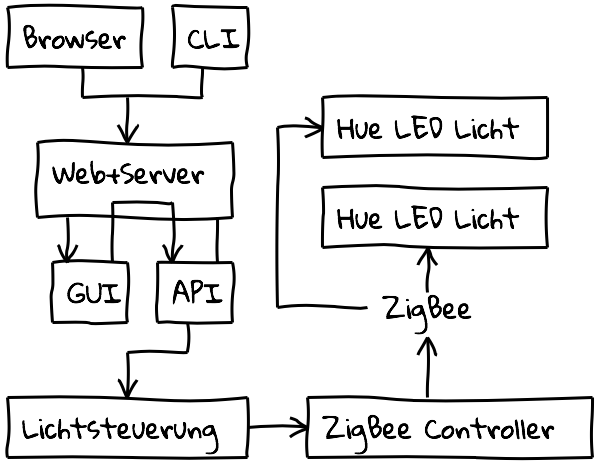
\includegraphics[width=0.9\linewidth]{img/grobarchitektur}
	\caption{Kommunikationsablauf der Komponenten}
	\label{fig:architecture}
\end{figure}

\noindent
Die Lichtsteuerung soll aus mehreren miteinander interagierenden Komponenten
bestehen, welche im Weiteren genauer beschrieben werden.

\subsection{Hue LED Licht}

Die Lampen, welche gesteuert werden sollen, werden in eine herkömmliche Fassung
geschraubt worüber sie wie normale Leuchtmittel mit Strom versorgt werden. Die Hue LEDs
besitzen außerdem einen ZigBee-Chip, mit dem sie Teil eines ZigBee-Netzwerks werden
können. In diesem Netzwerk arbeiten sie als \emph{End Device}. Über das ZigBee
\emph{Light Link}-Protokoll können die Lampen angesprochen werden und bestimmte
Einstellungen wie Helligkeit und Farbe eingestellt werden.

\newpage

\subsection{ZigBee Controller}

Der ZigBee Controller ist die eigentliche Funkeinheit. Sie stellt eine rohe
Programmierschnittstelle bereit, um auf das ZigBee-Netzwerk zugreifen zu können.

\begin{figure}[h!]
	\centering
	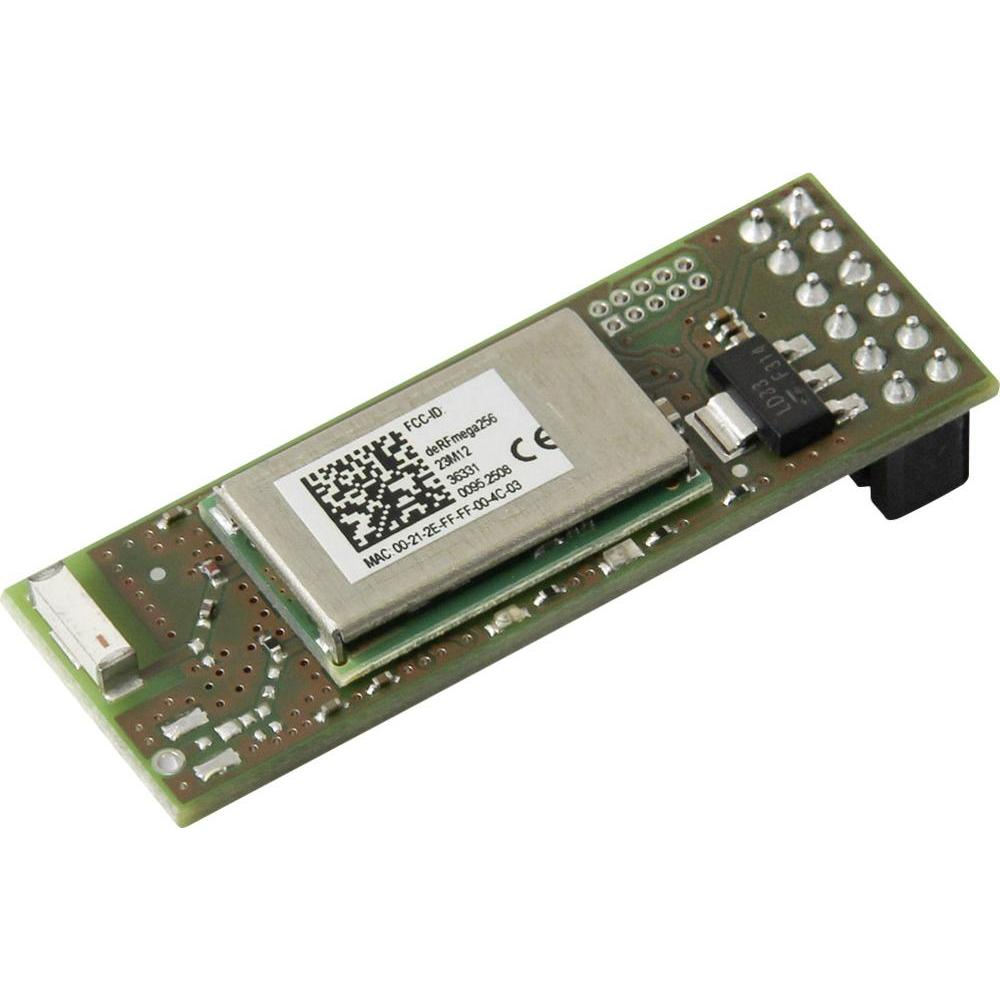
\includegraphics[width=0.4\linewidth]{img/raspbee}
	\caption{RaspBee-Funkmodul}
\end{figure}

Der Controller besteht aus zwei Komponenten. Zum einen dem \emph{RaspBee}, eine
aufsteckbare Erweiterungsplatine mit Funkmodul für \emph{Raspberry Pi}, und zum
anderen dem \emph{Raspberry Pi} selber. Der \emph{Raspberry Pi}, ein
Entwicklungsboard, besitzt eine Reihe an GPIO Pins am Rand des Boards.

\begin{figure}[h!]
	\centering
	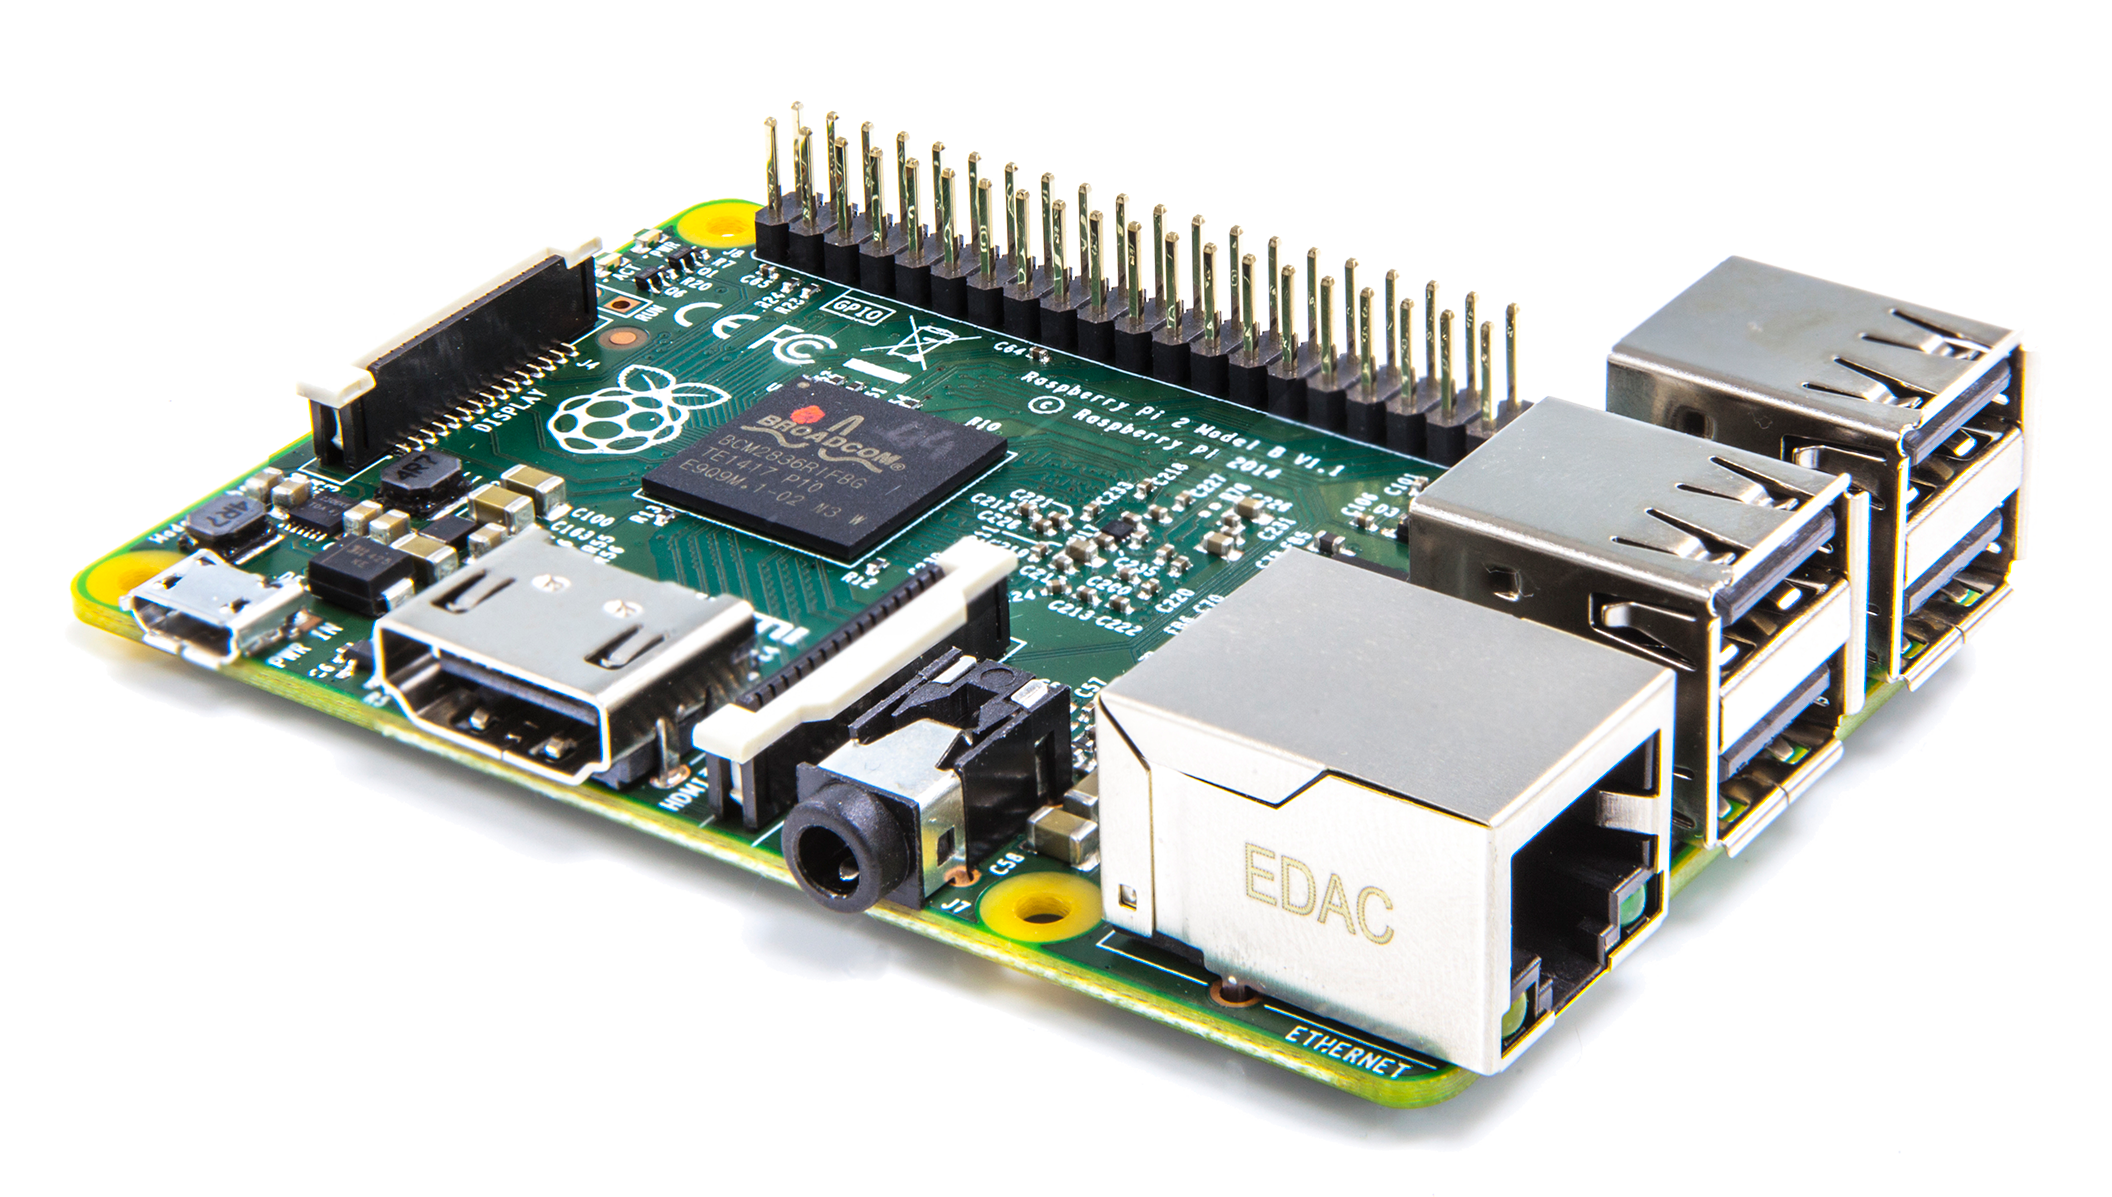
\includegraphics[width=0.7\linewidth]{img/rpi2}
	\caption{Raspberry 2}
\end{figure}

Das \emph{RaspBee} ist an diese GPIO Pins angepasst und wird dadurch mit Strom gespeist.
Weiterhin werden die \emph{UART}-Pins zur seriellen Kommunikation mit einem
Treiber, der auf dem \emph{Raspberry Pi} betrieben wird, verwendet.

\subsection{Lichtsteuerung}

Die Lichtsteuerung dient als hardwarenahes Backend. Diese Software, welche auf
dem \emph{Raspberry Pi} betrieben wird, kommuniziert über die serielle
Schnittstelle mit dem ZigBee Controller. Um auf die Nodes des Netzwerks
zugreifen zu können bietet das Backend eine Programmierschnittstelle an.

\subsection{API}

Die API ist eine weitere Software auf dem \emph{Raspberry Pi}. Sie verwendet
die Schnittstelle der Lichtsteuerung und bietet eine REST-basierte
Webschnittstelle an. Diese Schnittstelle bietet einen vereinfachten Zugriff
auf das Funknetz, mit Fokus auf Steuerung und Verwaltung der Lampen. Durch die
Trennung der einzelnen Programme bleiben Treiber, API und GUI austauschbar.

\subsection{Webserver}

Der Webserver dient primär zum Zugriff auf die Web-GUI, welche die REST-API
über den Browser zugänglich macht um bequem die Lichter verwalten und steuern
zu können. Weiter wird hier die API etwaigen CLI-Programmen zur Verfügung
gestellt.

\subsection{GUI}

Die GUI, im HTML5 Standard, ist die Schnittstelle zum Benutzer und wird im Browser dargestellt.
Über diese kann der Benutzer die Nodes steuern, wie z.B. Helligkeit und Farbe einstellen.
Zum bequemen Verwenden der API aus dem Browser wird JavaScript auf dem Client verwendet. 

\subsection{CLI}

Um die Lampensteuerung automatisieren zu können, etwa um aus dem Urlaub oder
zeitgesteuert in seinem Haus das Licht aus- oder anzuschalten, ist ein
Kommandozeileninterface wünschenswert. Für viele Sprachen gibt es bereits
Module mit denen REST-APIs angesprochen werden können, daher ist die
Programmiersprache in der das CLI-Programm umgesetzt werden soll zweitrangig.

\newpage

\section{Umsetzung}
\label{doing}

Umgesetzt und von uns implementiert werden soll die API sowie die CLI. Eine
rudimentäre Umsetzung der Web-GUI ist auch denkbar um die prinzipielle
Möglichkeit zu verdeutlichen.

Die Treibersoftware um das \emph{RaspBee}-Modul anzusteuern ist leider nicht
Open Source. Diese Software bietet eine Programmierschnittstelle, um welche
wir unsere API herum entwickeln können. Der \emph{RaspBee}-Hersteller hat auf
Nachfrage bestätigt, dass weder die UART-Spezifikation, noch der Quellcode
des Treibers öffentlich sei. Da ein Reverse-Engineering des Treibers den Rahmen
des Projekts sprengen würde haben wir uns darauf geeinigt, die Software des
Herstellers zu verwenden.

\subsection{Einschränkungen}

Nach anfänglicher Exploration der mit der \emph{RaspBee}-Modul zugehörigen Software
von \emph{Dresden Elektronik} wurde festgestellt, dass viel der von uns zu
implementierenden Funktionalität bereits vorhanden war. Die Anfrage an den
Support von \emph{Dresden Elektronik} nach Zugang zur Dokumentation der
\emph{UART}-Schnittstelle und dem Funkmodul wurde verweigert.

Weiter war das Vorhaben aus Punkt \ref{architecture} inhaltlich zu groß gefasst
als dass es in der gegebenen Zeit vollumfänglich durchgeführt werden könnte.

\end{document}